\documentclass[twoside]{article}
\usepackage[a4paper]{geometry}
\geometry{verbose,tmargin=2.5cm,bmargin=2cm,lmargin=2cm,rmargin=2cm}
\usepackage{fancyhdr}
\pagestyle{fancy}

% nastavení pisma a~češtiny
\usepackage{lmodern}
\usepackage[T1]{fontenc}
\usepackage[utf8]{inputenc}
\usepackage[czech]{babel}

% odkazy
\usepackage{url}

\usepackage{float}
% vícesloupcové tabulky
\usepackage{multirow}
\usepackage{listings}
\usepackage{xcolor}
\usepackage{amssymb}
\usepackage{gensymb}
\usepackage{bbold}
\usepackage{amsmath}
\usepackage{siunitx}
\usepackage{mathtools}
\usepackage{commath}

% vnořené popisky obrázků
\usepackage{subcaption}

% automatická konverze EPS 
\usepackage{graphicx} 
\usepackage{epstopdf}
\epstopdfsetup{update}

\graphicspath{{./images}}

% odkazy a~záložky
\usepackage[unicode=true, bookmarks=true,bookmarksnumbered=true,
bookmarksopen=false, breaklinks=false,pdfborder={0 0 0},
pdfpagemode=UseNone,backref=false,colorlinks=true] {hyperref}


% Poznámky při překladu
\usepackage{xkeyval}	% Inline todonotes
\usepackage[textsize = footnotesize]{todonotes}
\presetkeys{todonotes}{inline}{}

%https://tex.stackexchange.com/questions/2783/bold-calligraphic-typeface
\DeclareMathAlphabet\mathbfcal{OMS}{cmsy}{b}{n}

% enumerate zacina s pismenem
\renewcommand{\theenumi}{\alph{enumi}}

% smaz aktualni page layout
\fancyhf{}
% zahlavi
\usepackage{titling}
\fancyhf[HC]{\thetitle}
\fancyhf[HLE,HRO]{\theauthor}
\fancyhf[HRE,HLO]{\today}
 %zapati
\fancyhf[FLE,FRO]{\thepage}

% údaje o autorovi
\title{OTE Domácí úkol 3a - Rozdílový zesilovač}
\author{Vojtěch Michal}
\date{\today}

%customize code listing
\definecolor{codegreen}{rgb}{0,0.6,0}
\definecolor{codegray}{rgb}{0.5,0.5,0.5}
\definecolor{codepurple}{rgb}{0.58,0,0.82}
\definecolor{backcolour}{rgb}{0.95,0.95,0.92}

\lstdefinestyle{mystyle}{
    backgroundcolor=\color{backcolour},   
    commentstyle=\color{codegreen},
    keywordstyle=\color{magenta},
    numberstyle=\tiny\color{codegray},
    stringstyle=\color{codepurple},
    basicstyle=\ttfamily\footnotesize,
    breakatwhitespace=false,         
    breaklines=true,                 
    captionpos=b,                    
    keepspaces=true,                 
    numbers=left,                    
    numbersep=5pt,                  
    showspaces=false,                
    showstringspaces=false,
    showtabs=false,                  
    tabsize=2
}

\lstset{style=mystyle}

\begin{document}

\maketitle

V simulacích pro tuto úlohu bylo použito nastavení parametrů operačního zesilovače uvedené v tabulce \ref{tab:oz_param}.
Symbolem $u_3$ označuji napětí na výstupu operačního zesilovače proti zemi,
napětí $u_2$ a $u_1$ jsou po řadě napětí kladného a záporného vstupu rozdílového zesilovače proti zemi
(konvence použitá v zadání).

\begin{table}[h!]
    \centering
    \begin{tabular}{c|c|c|c|c}
        parametr & symbol & hodnota & jednotka & poznámka\\
        \hline
        Vstupní napěťový offset & $U_0$ & 1 & \si{\milli\volt} & \\
        Vstupní klidový proud & $I_\text{B}$ & 50 & \si{\nano\ampere} & $(I_\text{BP} + I_\text{BN})/2$ \\
        Vstupní zbytkový proud & $I_0$ & 20 & \si{\nano\ampere} & $I_\text{BP} - I_\text{BN}$ \\
        Zesílení v otevřené smyčce & $A_\text{D}$ & 200 & \si{\kilo\volt\per\volt} & \\
        Tranzitní kmitočet& $f_T$ & 1 & \si{\mega\hertz} &
    \end{tabular}
    \caption{Parametry operačního zesilovače použité pro simulaci}
    \label{tab:oz_param}
\end{table}

\section{Zbytková napětí}

\begin{figure}[h!]
    \centering
    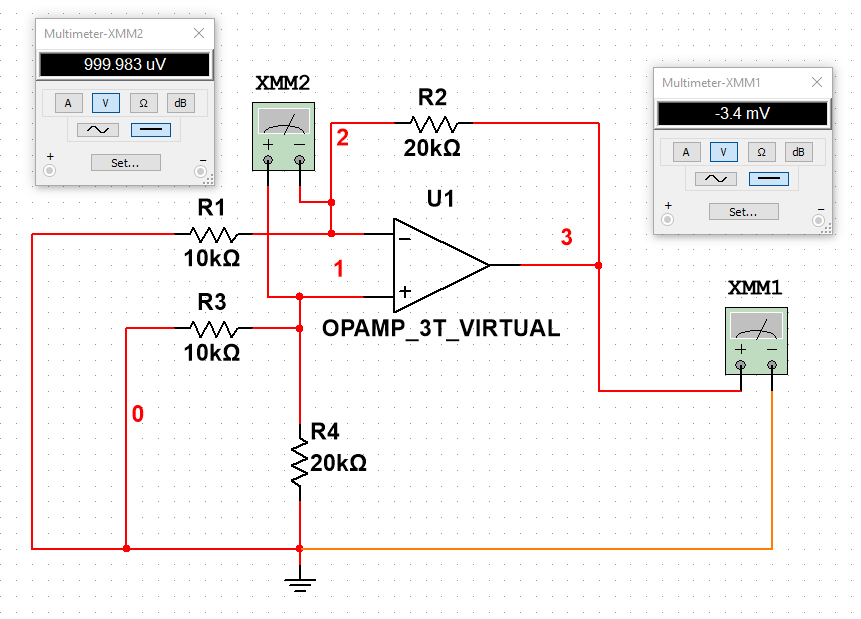
\includegraphics[width=0.5\linewidth]{rozdilovy_zbytkove_napeti.png}
    \caption{Zapojení pro změření zbytkového výstupního napětí rozdílového zesilovače}
    \label{fig:zbytkove_u}
\end{figure}

Multimetrem byly změřeny hodnoty zbytkových výstupních napětí uvedené v tabulce \ref{tab:zbytkova_u},
použité zapojení je na obrázku \ref{fig:zbytkove_u}.

\begin{table}[h!]
    \centering
    \begin{tabular}{c|c}
        jmenovité rozdílové zesílení $G_\text{D}$ & výstupní zbytkové napětí \\
        \hline
        2 & -3,4 \si{\milli\volt} \\
        4 & -5,8 \si{\milli\volt} \\
        8 & -10,6 \si{\milli\volt} \\
        16 & -20,2 \si{\milli\volt}
    \end{tabular}
    \caption{Naměřená výstupní zbytková napětí rozdílového zesilovače v závislosti na zesílení}
    \label{tab:zbytkova_u}
\end{table}

\subsection{Odvození vstupních zbytkových napětí}

Předpokládám $u_1 = u_3 = 0 \si{\volt}$. Kvůli klidovému proudu $I_\text{BN}$ je napětí na invertující
svorce OZ rovno
\begin{equation}
    u_- = - (R_1 \vert \vert R_2) I_\text{BN} =  - \frac{R_1 R_2}{R_1 + R_2} I_\text{BN}.
\end{equation}
Aby byl splněn předpoklad $u_3 = 0 \si{\volt}$, potřebuji na neinvertující vstup dostat napětí
\begin{equation}
    u_+ = u_- + U_0,
\end{equation}
kde $U_0$ je vstupní zbytkové napětí samotného OZ dle \ref{tab:oz_param}.
Protože dále dle Kirchhoffova zákona proudů, aplikovaného na uzel u neinvertující svorky, platí 
\begin{equation}
    \begin{split}
        \frac{u_2 - u_+}{R_3} &= I_\text{BP} + \frac{u_+}{R_4}, \\
        u_2 &= u_+ + R_3 (I_\text{BP} + \frac{u_+}{R_4}), \\
        u_2 &= R_3 I_\text{BP} + \frac{R_3 + R_4}{R_4}u_+,
    \end{split}
\end{equation}
je vstupní zbytkové napětí rozdílového zesilovače rovno
\begin{equation}
    u_2 = R_3 I_\text{BP} + \frac{R_3 + R_4}{R_4} (U_0 - \frac{R_1 R_2}{R_1 + R_2} I_\text{BN}).
\end{equation}
S použitím diagonalizační podmínky $R_1 = R_3$ a $R_2 = R_4$ po úpravách platí
\begin{equation}
    \begin{split}
        u_2 = R_1 I_\text{BP} + \frac{R_1 + R_2}{R_2} (U_0 - \frac{R_1 R_2}{R_1 + R_2} I_\text{BN}), \\
        u_2 = R_1 I_\text{BP} + \frac{R_1 + R_2}{R_2} U_0 - R_1 I_\text{BN}. \\
    \end{split}
    \label{eq:zbytkove_u}
\end{equation}
Výsledky dosazení různých hodnot odporu $R_2$ do rovnice \eqref{eq:zbytkove_u} jsou v tabulce \ref{tab:vstupni_zbytkova_u},
kde jsou porovnány s hodnotami ze simulací při fixovaném $R_1 = 10 \si{\kilo\ohm}$. Výpočty byly prováděné v prostředí
\textit{MATLAB} vyhodnocením výrazu \textit{R2 = 10e3; R1 = 10e3; IBP = 60e-9; IBN = 40e-9; U0 = 1e-3; R1 * IBP + (R1 + R2) / R2 * U0 - R1 * IBN}.
Simulačně bylo vstupní zbytkové napětí získáno zapojením záporné zpětné vazby dle schématu \ref{fig:vstupni_zbytkove}
regulující výstupní napětí rozdílového zesilovače na nulu. Vypočtená napětí dokonale odpovídají výsledkům simulace.

\begin{table}[h!]
    \centering
    \begin{tabular}{c|c|c}
        $R_2$ [\si{\kilo\ohm}] & vypočtené vstupní zbytkové U & simulované vstupní zbytkové U \\
        \hline
        10 & 2,2 \si{\milli\volt} & 2,2 \si{\milli\volt} \\
        20 & 1,7 \si{\milli\volt} & 1,7 \si{\milli\volt} \\
        40 & 1,45 \si{\milli\volt} & 1,45 \si{\milli\volt} \\
        80 & 1,325 \si{\milli\volt} & 1,325 \si{\milli\volt} \\
        160 & 1,26 \si{\milli\volt} & 1,263 \si{\milli\volt} \\
    \end{tabular}
    \caption{Vypočítaná a změřená vstupní zbytková napětí rozdílového zesilovače}
    \label{tab:vstupni_zbytkova_u}
\end{table}

\begin{figure}[h!]
    \centering
    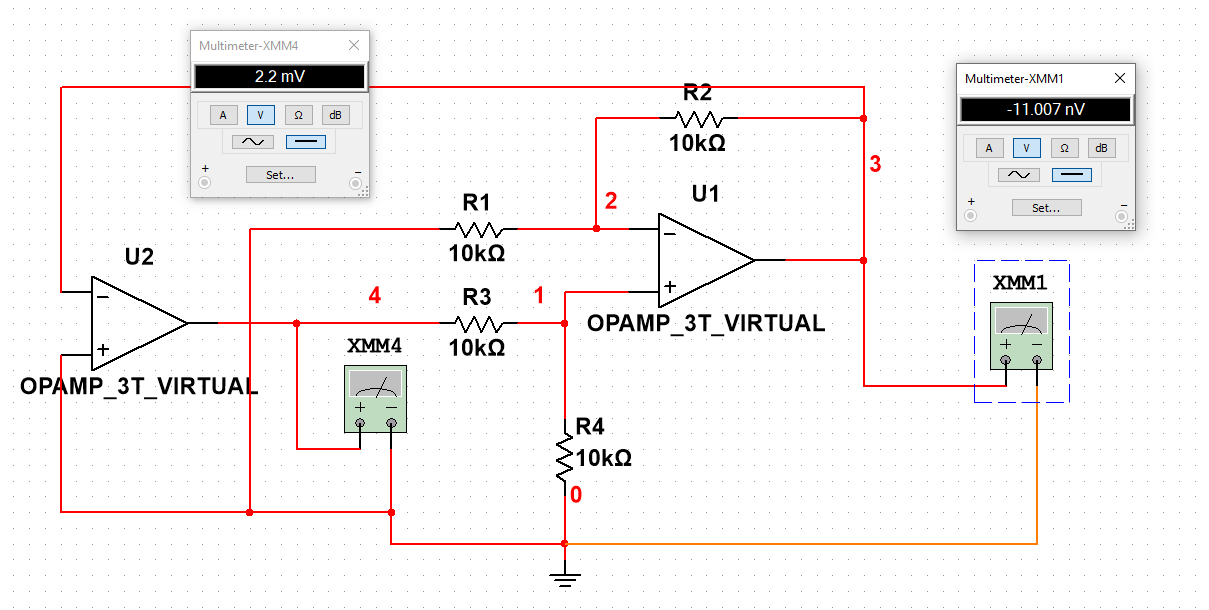
\includegraphics[width=0.6\linewidth]{vstupni_zbytkove.png}
    \caption{Zpětnovazební zapojení pro zjištění vstupního zbytkového napětí rozdílového zesilovače}
    \label{fig:vstupni_zbytkove}
\end{figure}

\section{Frekvenční charakteristika rozdílového zesílení $G_\text{D}$}

S pomocí zapojení na schématu \ref{fig:schema_diff_bode} a funkce \textit{AC sweep} byly
získány frekvenční charakteristiky rozdílového zesílení pro $G_\text{D} \in \left\{4, 16\right\}$,
které jsou vykresleny na obrázkách \ref{fig:bode_diff_4} a \ref{fig:bode_diff_16}.
Mezní kmitočty pro jednotlivá rozdílová zesílení jsou zanesena v tabulce \ref{tab:mezni_f}
a odpovídají analytickému vztahu pro \textit{gain-bandwidth product} $f_m \cdot (G_\text{D} + 1) = f_T$.

\begin{figure}[h!]
    \centering
    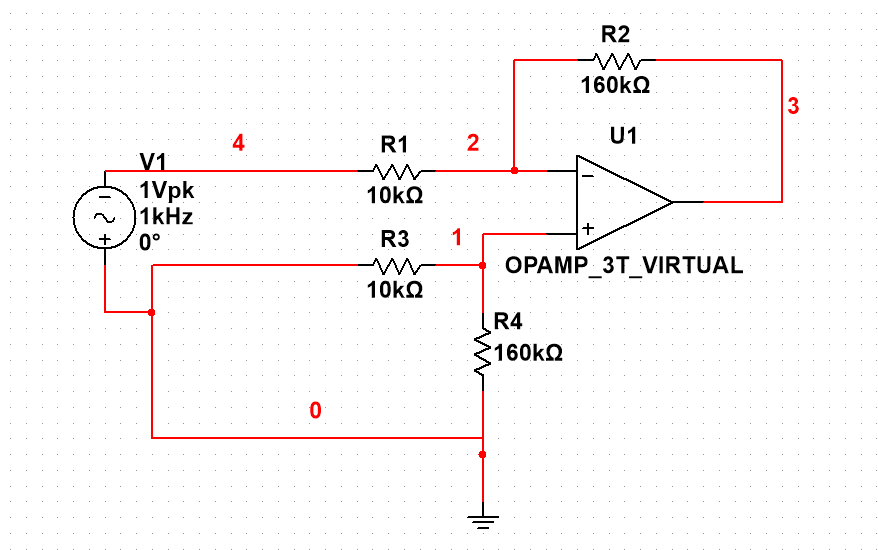
\includegraphics[width=0.8\linewidth]{rozdilovy_diff.png}
    \caption{Zapojení pro získání frekvenční charakteristiky rozdílového zesílení $G_\text{D}$}
    \label{fig:schema_diff_bode}
\end{figure}

\begin{table}[h!]
    \centering
    \begin{tabular}{c|c}
        rozdílové zesílení $G_\text{D}$ & mezní kmitočet $f_m$ [\si{\kilo\hertz}] \\
        \hline
        1 & 500 \\
        2 & 330 \\
        4 & 200 \\
        8 & 112 \\
        16 & 58
    \end{tabular}
    \caption{Závislost mezní frekvence na rozdílovém zesílení}
    \label{tab:mezni_f}
\end{table}

\begin{figure}[h!]
    \centering
    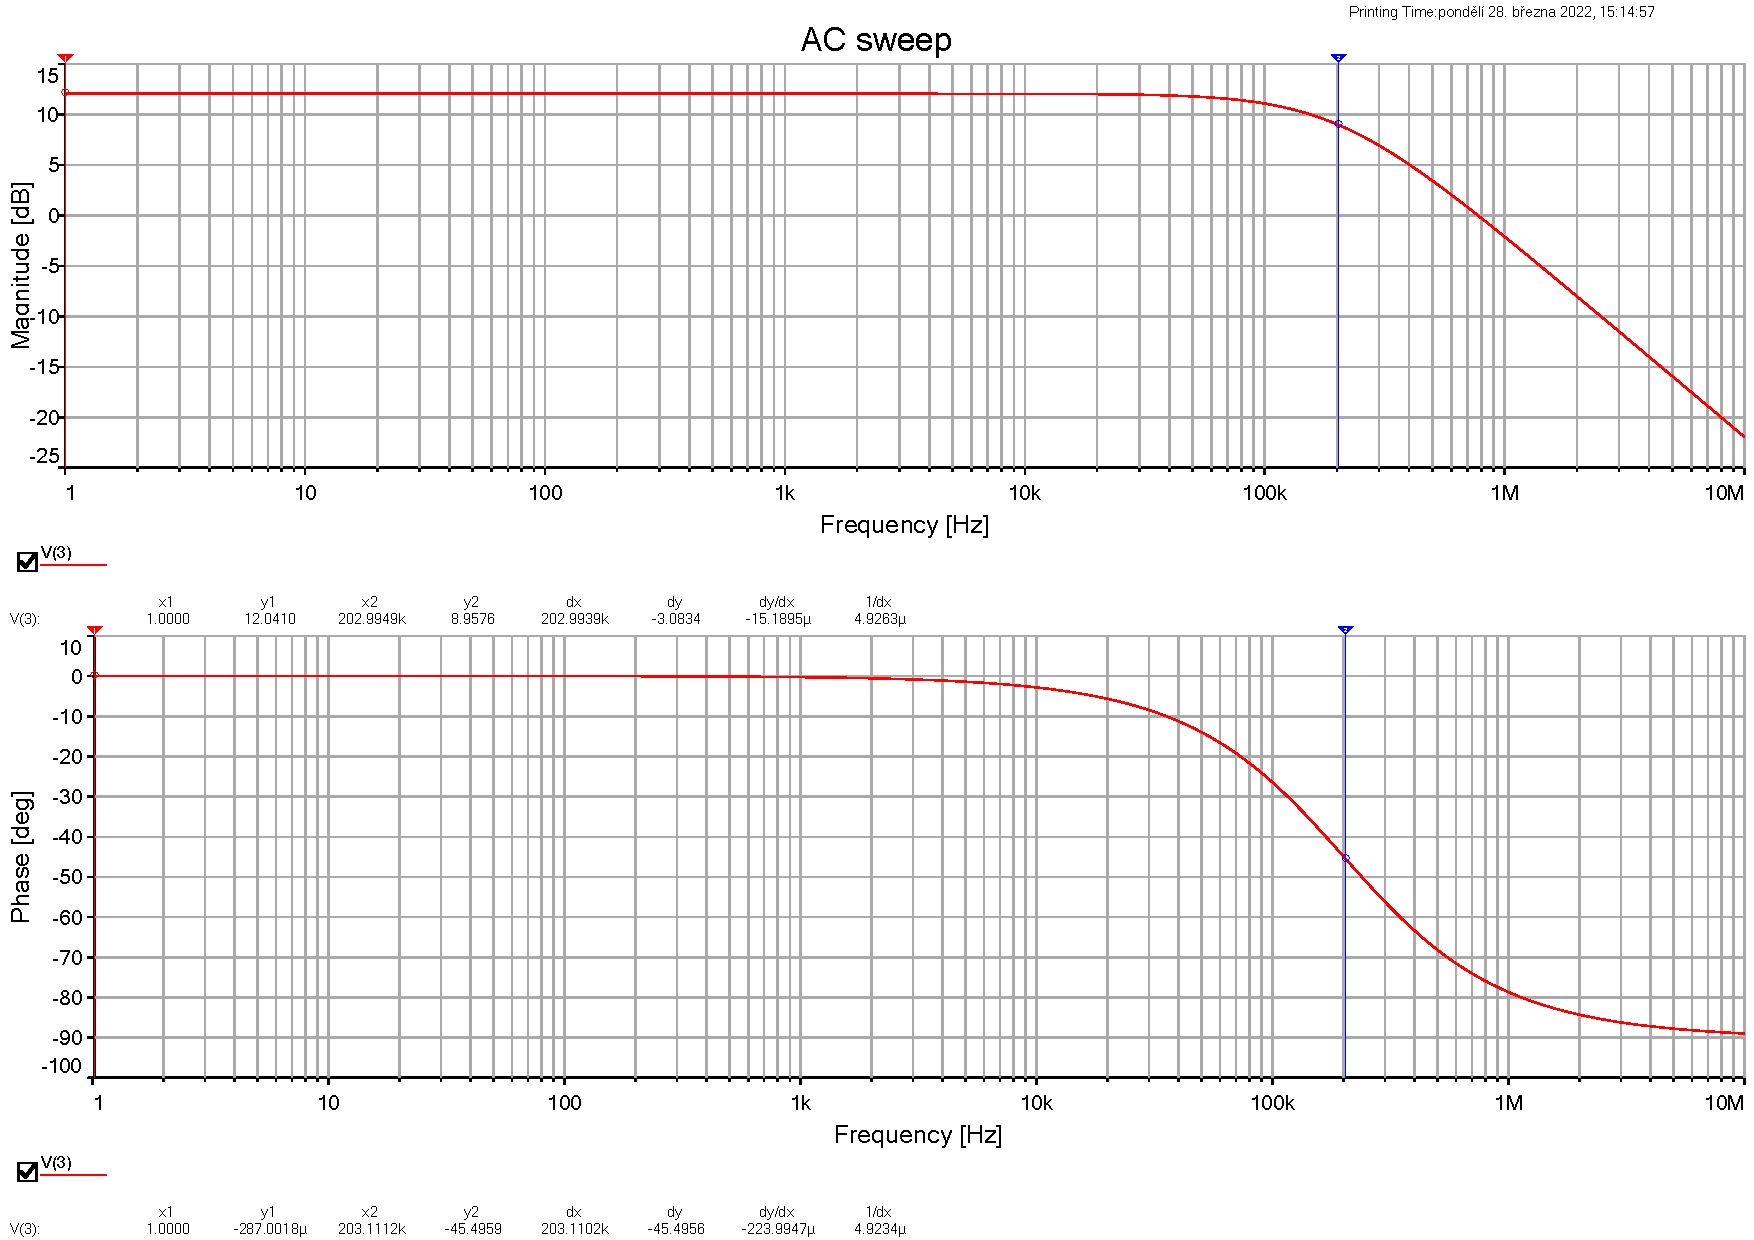
\includegraphics[width=0.92\linewidth]{bode_diff_4.pdf}
    \caption{Frekvenční charakteristika rozdílového zesílení pro $G_\text{D} = 4$}
    \label{fig:bode_diff_4}
\end{figure}

\begin{figure}[h!]
    \centering
    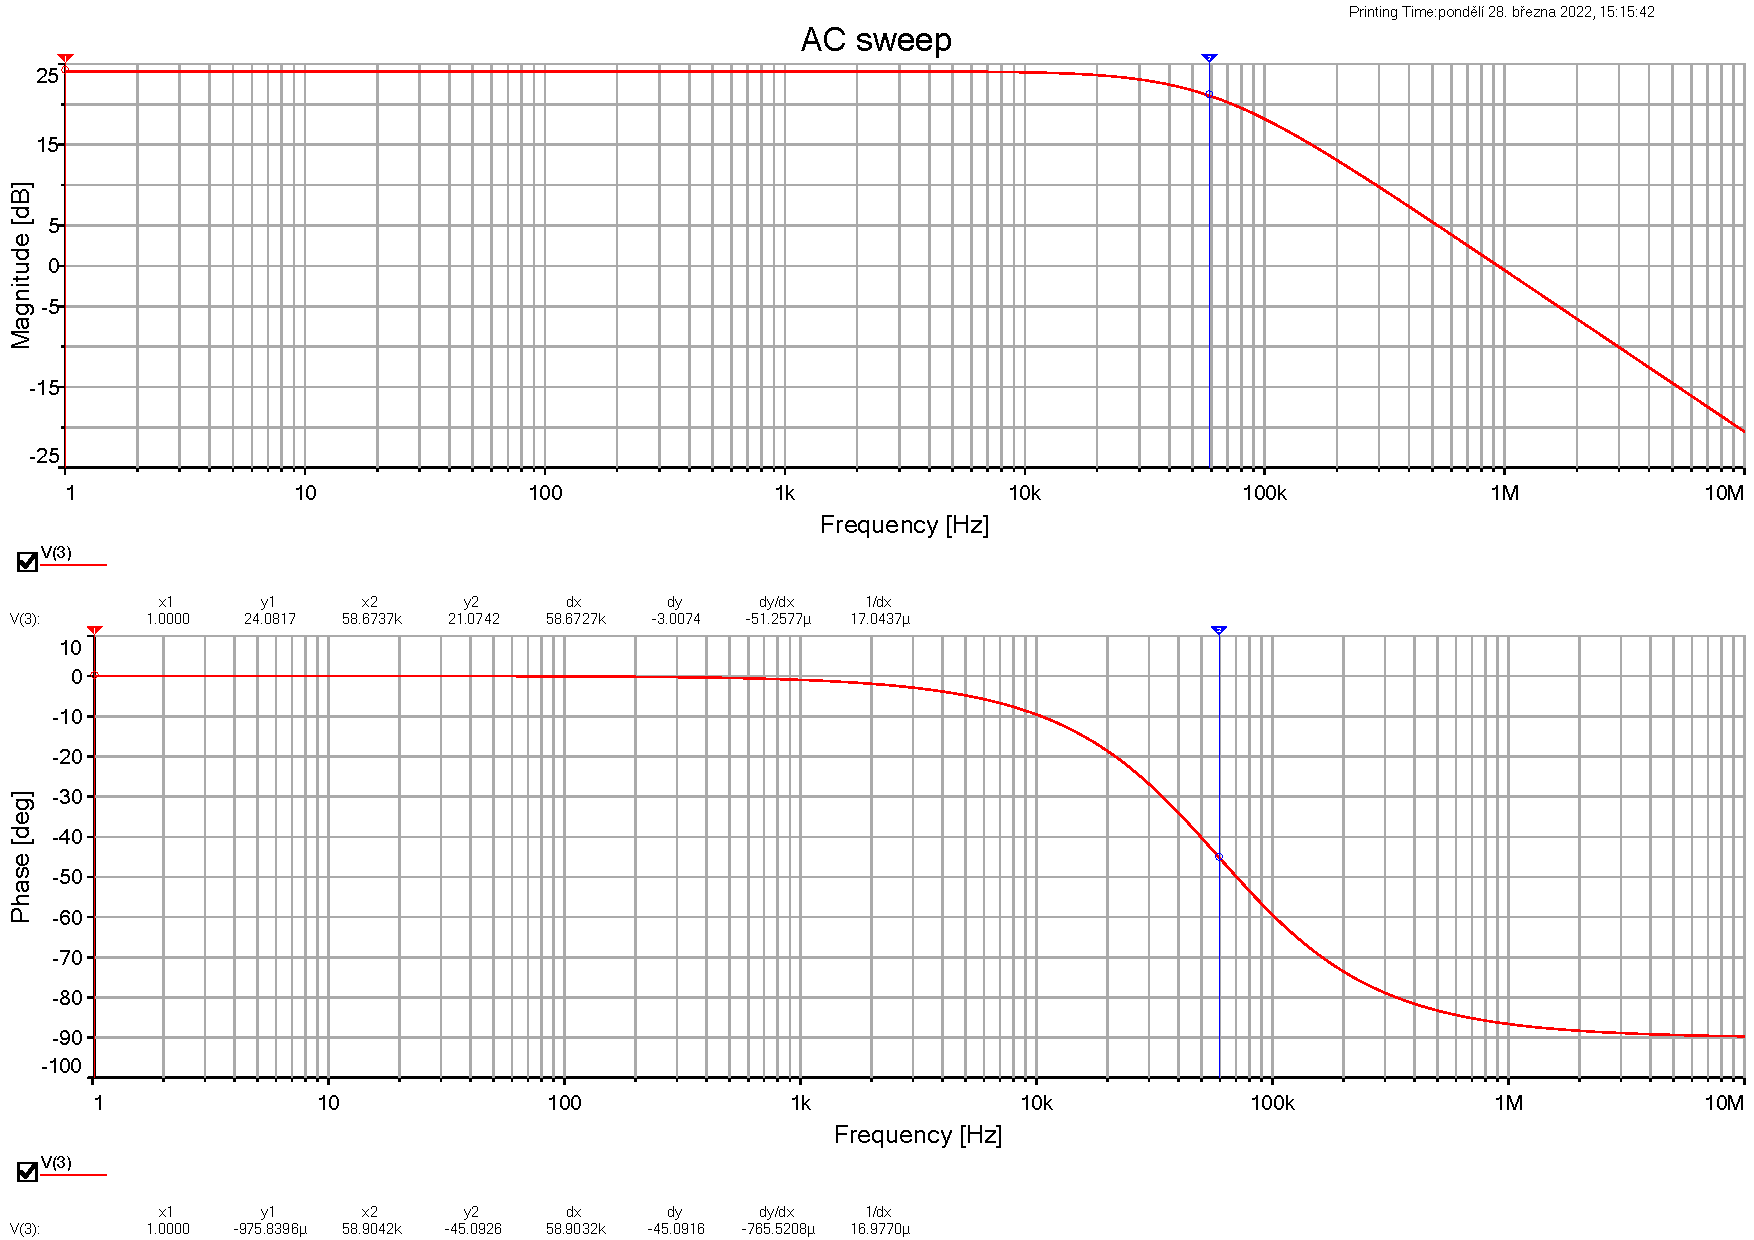
\includegraphics[width=0.92\linewidth]{bode_diff_16.pdf}
    \caption{Frekvenční charakteristika rozdílového zesílení pro $G_\text{D} = 16$}
    \label{fig:bode_diff_16}
\end{figure}

\newpage
\section{Frekvenční charakteristika souhlasného zesílení $G_\text{C}$}

\begin{figure}[h!]
    \centering
    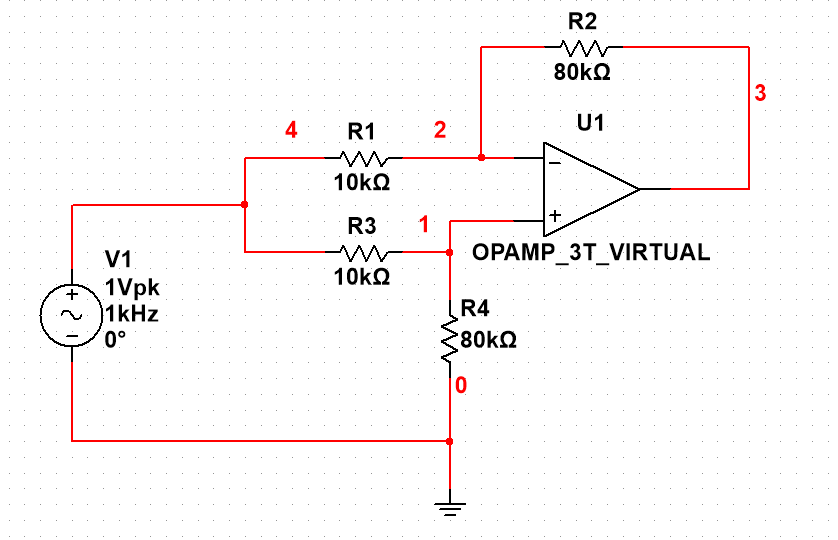
\includegraphics[width=0.8\linewidth]{rozdilovy_common_mode.png}
    \caption{Zapojení pro získání frekvenční charakteristiky souhlasného zesílení $G_\text{C}$}
    \label{fig:schema_common}
\end{figure}


S pomocí zapojení na schématu \ref{fig:schema_common} a funkce \textit{AC sweep} byly
získány frekvenční charakteristiky souhlasného zesílení pro $G_\text{D} \in \left\{4, 16\right\}$,
které jsou vykresleny na obrázkách \ref{fig:bode_common_4} a \ref{fig:bode_common_16}.

Mezní kmitočty jsou stejné jako u rozdílových zesílení (viz tabulka \ref{tab:mezni_f}),
frekvenční charakteristika má derivační charakter - vyšší kmitočty jsou propouštěny lépe
než nižší. Srovnání CMRR pro různá zesílení a frekvence je v tabulce \ref{tab:CMRR}.
Hodnoty souhlasného zesílení $G_\text{C}$ jsou uvedeny v decibelech a tedy platí 
$\text{CMRR} = G_\text{D} - G_\text{C}$.

\begin{table}[h!]
    \centering
    \begin{tabular}{c|c|c}
        & $G_\text{D} = 12 \si{\deci\bel}$ & $G_\text{D} = 24 \si{\deci\bel}$ \\ \hline
        $f \to 0$ & -152 dB & -136 dB \\
        $f \to \infty$ & -73 dB & -85 dB
    \end{tabular}
    \caption{Závislost souhlasného zesílení $G_\text{C}$ na frekvenci $f$ a $G_\text{D}$}
    \label{tab:CMRR}
\end{table}

Stejnosměrné souhlasné rušení lépe potlačuje méně zesilující rozdílový zesilovač
(pro $G_\text{D} = 4 = 12 \si{\deci\bel}$ je $\text{CMRR} = 164 \si{\deci\bel}$),
naopak na vyšších frekvencích léep potlačuje více zesilující zesilovač 
(pro $G_\text{D} = 16 = 24 \si{\deci\bel}$ je $\text{CMRR} = 109 \si{\deci\bel}$).

\begin{figure}[h!]
    \centering
    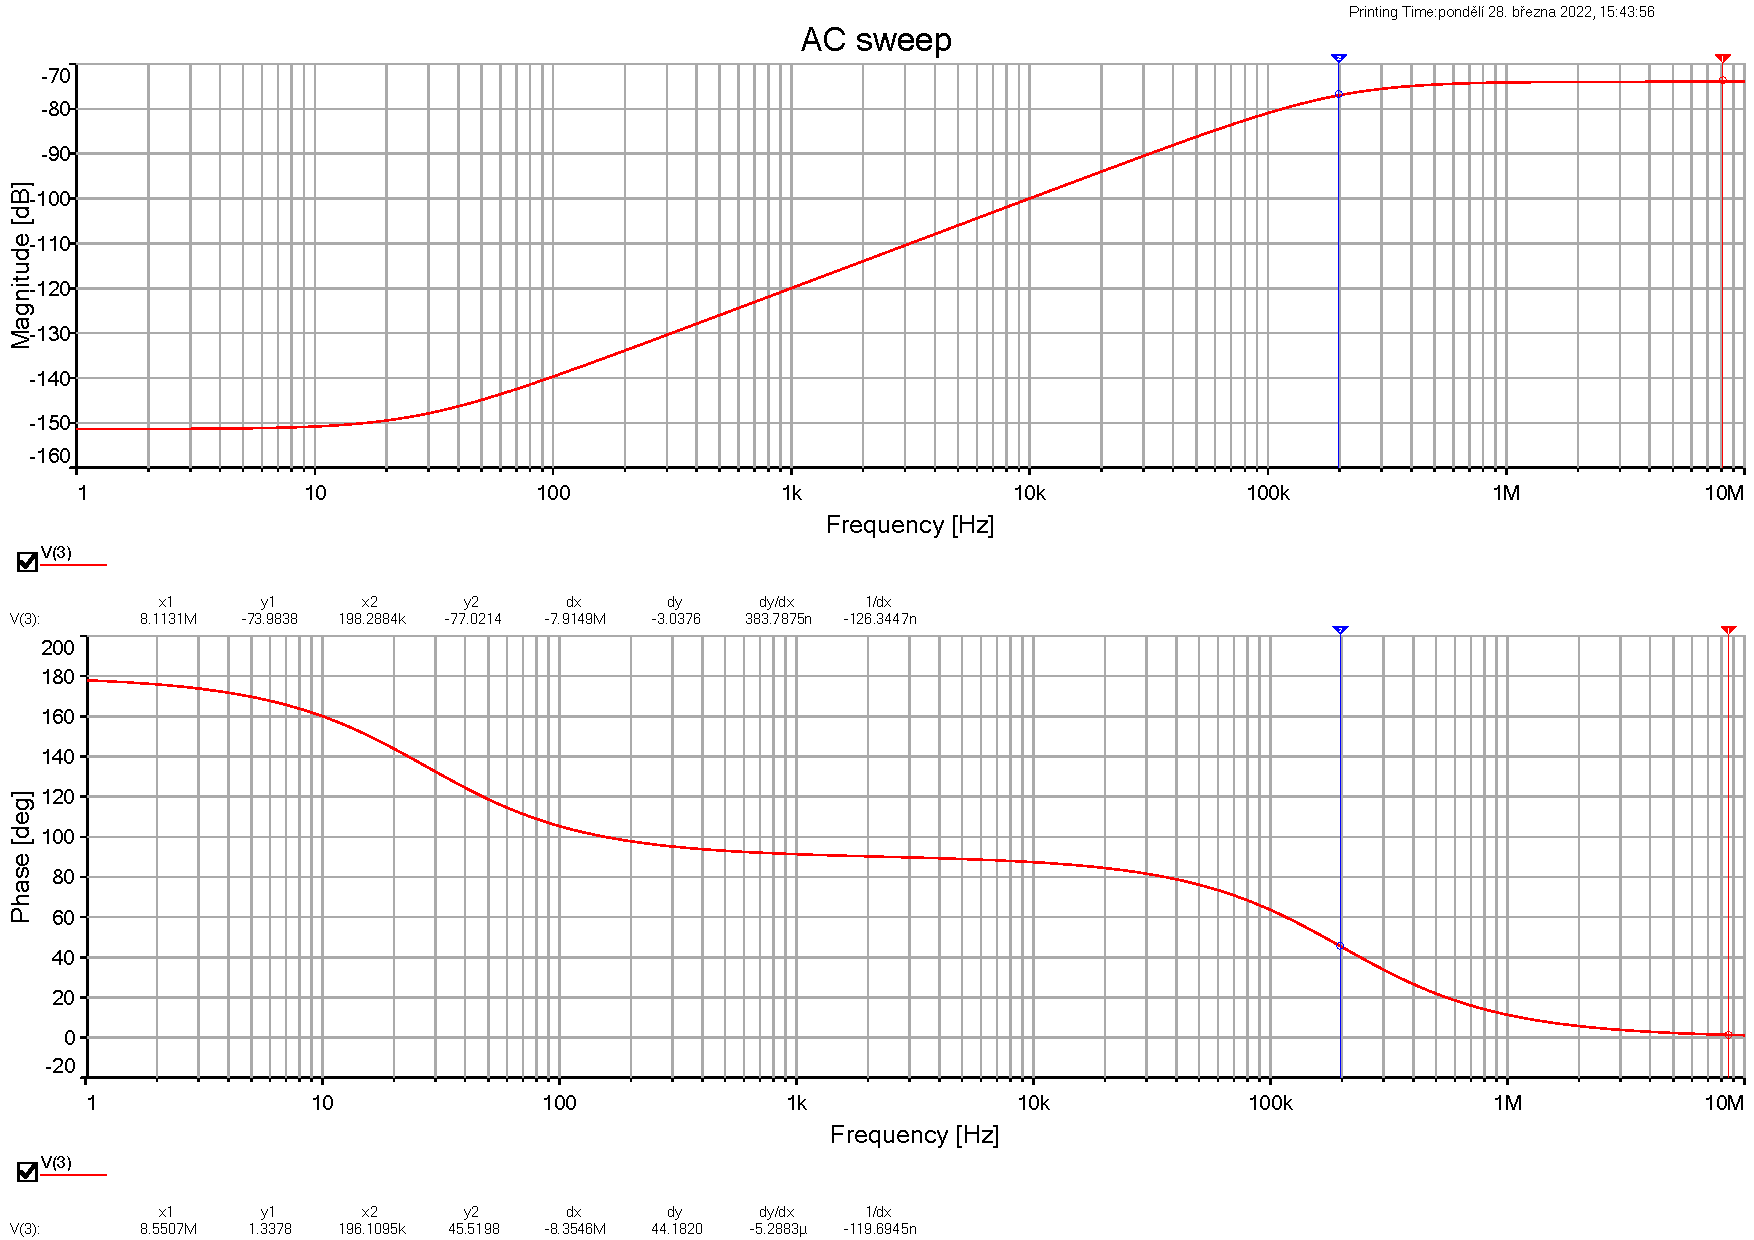
\includegraphics[width=0.92\linewidth]{bode_common_4.pdf}
    \caption{Frekvenční charakteristika souhlasného zesílení pro $G_\text{D} = 4$}
    \label{fig:bode_common_4}
\end{figure}

\begin{figure}[h!]
    \centering
    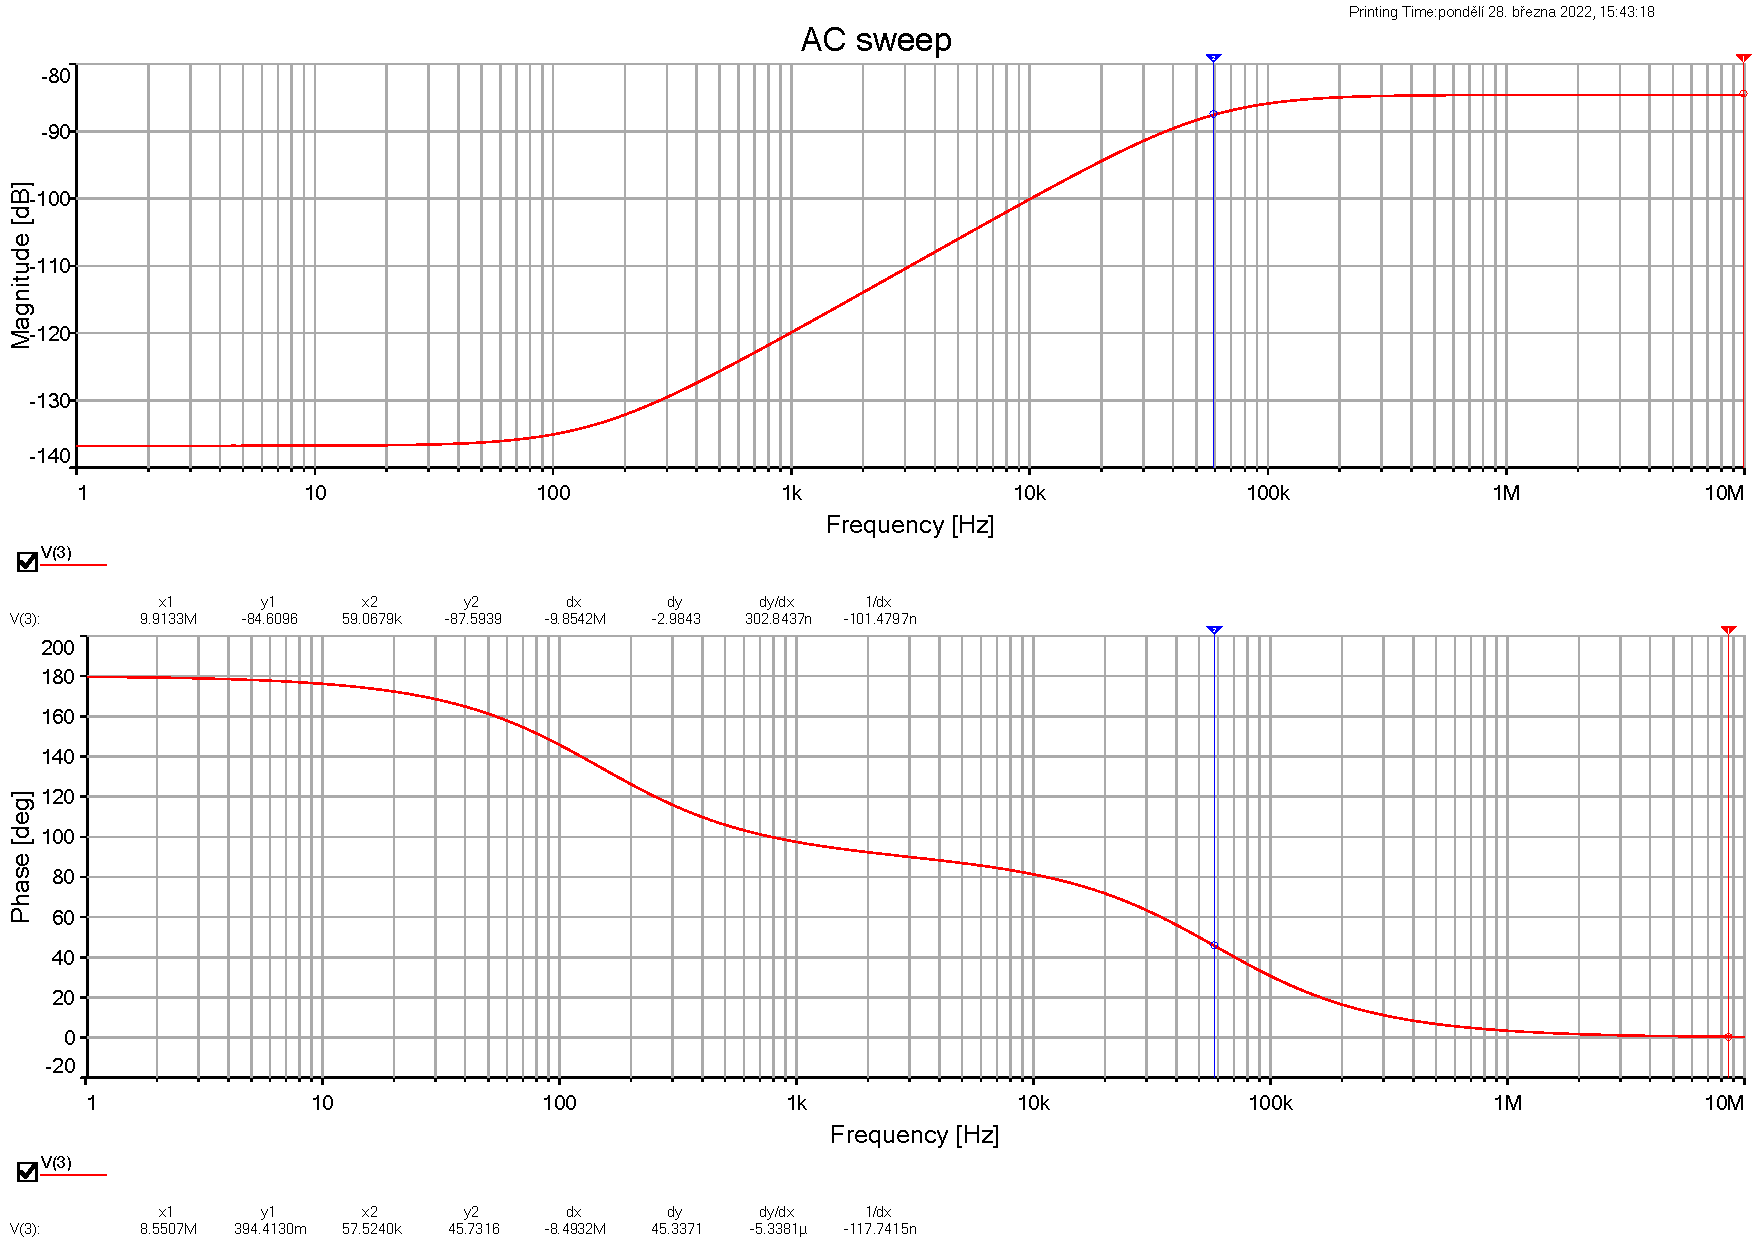
\includegraphics[width=0.92\linewidth]{bode_common_16.pdf}
    \caption{Frekvenční charakteristika souhlasného zesílení pro $G_\text{D} = 16$}
    \label{fig:bode_common_16}
\end{figure}
\newpage

\section{Doba náběhu}

\begin{figure}[h!]
    \centering
    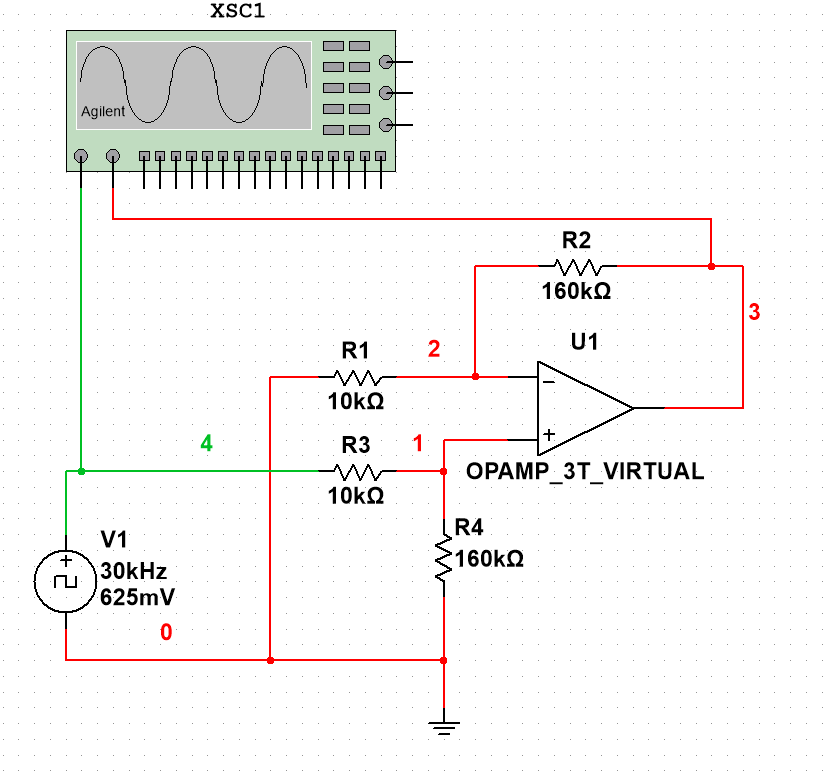
\includegraphics[width=0.7\linewidth]{rise_time_schema.png}
    \caption{Zapojení pro měření doby náběhu}
    \label{fig:rise_time_schema}
\end{figure}

S pomocí generátoru obdélníkového signálu a osciloskopu zapojeného dle schématu \ref{fig:rise_time_schema}
byly zachyceny časové průběhy vykreslené na obrázkách \ref{fig:rise_time_4} a \ref{fig:rise_time_16}.
Pomocí kurzorů byly odečteny doby náběhu $T_n = 1,858 \si{\micro\second}$ pro $G_\text{D} = 4$ a 
$T_n = 6,068 \si{\micro\second}$ pro $G_\text{D} = 16$. Oba odpovídají očekávaným
dobám náběhu vypočteným dle vztahu $T_n \approx 0,35 / f_m$.

\begin{figure}[h!]
    \centering
    \begin{subfigure}{0.45\textwidth}
        \centering
        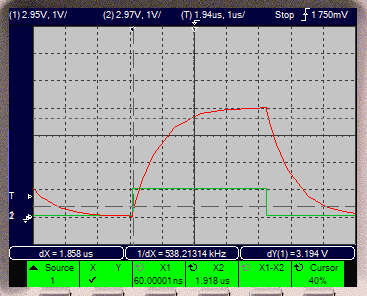
\includegraphics[width=0.8\linewidth]{rise_time_4.png}
        \caption{Pro $G_\text{D}=4$}
        \label{fig:rise_time_4}
    \end{subfigure}
    \begin{subfigure}{0.45\textwidth}
        \centering
        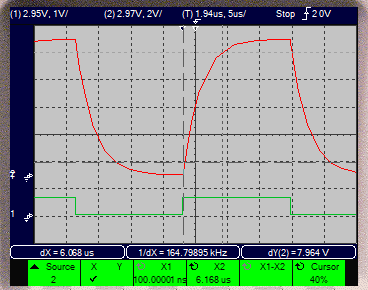
\includegraphics[width=0.8\linewidth]{rise_time_16.png}
        \caption{Pro $G_\text{D}=16$}
        \label{fig:rise_time_16}
    \end{subfigure}
    \caption{Měření doby náběhu $T_n$ rozdílového zesilovače}
\end{figure}

\end{document}

